% !TEX TS-program = xelatex

%%%%%%%%%%%%%%%%%%%%%%% 
% 文档类型,页面布局
\documentclass[UTF8,a4paper,10pt]{ctexart}
\usepackage[left=2.50cm, right=2.50cm, top=2.50cm, bottom=2.50cm]{geometry} %页边距
\CTEXsetup[format={\Large\bfseries}]{section} %设置章标题居左

%%%%%%%%%%%%%%%%%%%%%%% 
% 设置中文字体,用 xelatex 编译
% \setmainfont{Microsoft YaHei}  % 微软雅黑
% \setmainfont{YouYuan}  % 幼圆
% \setmainfont{NSimSun}  % 新宋体
% \setmainfont{KaiTi}    % 楷体
% \setmainfont{SimSun}   % 宋体
% \setmainfont{SimHei}   % 黑体

%%%%%%%%%%%%%%%%%%%%%%% 
% 设置英文字体
\usepackage{times}
% \usepackage{mathpazo}
% \usepackage{fourier}
% \usepackage{charter}
% \usepackage{helvet}

%%%%%%%%%%%%%%%%%%%%%%% 
% 各种包
\usepackage{amsmath, amsfonts, amssymb} % math equations, symbols
\usepackage[english]{babel}
\usepackage{color}      % color content
\usepackage{graphicx}   % import figures
\graphicspath{{figures/}}
\usepackage{url}        % hyperlinks
\usepackage{bm}         % bold type for equations
\usepackage{multirow} 	% multirow
\usepackage{booktabs}	% toprule,midrule,cmidrule,bootomrule
\usepackage{epstopdf}
\usepackage{epsfig}
\usepackage{algorithm}
\usepackage{algorithmic}
\renewcommand{\algorithmicrequire}{ \textbf{Input:}}     % use Input in the format of Algorithm
\renewcommand{\algorithmicensure}{ \textbf{Initialize:}} % use Initialize in the format of Algorithm
\renewcommand{\algorithmicreturn}{ \textbf{Output:}}     % use Output in the format of Algorithm
\usepackage{hyperref} %bookmarks
\hypersetup{colorlinks, bookmarks, unicode} %unicode

%%%%%%%%%%%%%%%%%%%%%%% 
% 设置页眉、页脚
\usepackage{fancyhdr}
% \pagestyle{fancy}
\lhead{}
\chead{}
% \rhead{\includegraphics[width=1.2cm]{fig/ZJU_BLUE.eps}}
\lfoot{}
\cfoot{}
\rfoot{}

%%%%%%%%%%%%%%%%%%%%%%% 
% 设置水印
% \usepackage{draftwatermark}         % 所有页加水印
% \usepackage[firstpage]{draftwatermark} % 只有第一页加水印
% \SetWatermarkText{Water-Mark}           % 设置水印内容
% \SetWatermarkText{\includegraphics{fig/ZJDX-WaterMark.eps}}         % 设置水印logo
% \SetWatermarkLightness{0.9}             % 设置水印透明度 0-1
% \SetWatermarkScale{1}                   % 设置水印大小 0-1


%%%%%%%%%%%%%%%%%%%%%%%%%%%%%%%%%%%%%%%%%%%%%%%%%%%%%%%%%%%%%%%%%%%%%%%%%%%%%%%% 
% 正文
%%%%%%%%%%%%%%%%%%%%%%%%%%%%%%%%%%%%%%%%%%%%%%%%%%%%%%%%%%%%%%%%%%%%%%%%%%%%%%%% 
\title{
  \textbf{位姿表示}
}
\author{石正璞
  % \thanks{学号:xx2017xxxx} 
}
\date{
  % \today
  2023年11月20日
}

\begin{document}
\maketitle	

\begin{abstract}
本文以笔记的形式对位姿的相关概念和算法进行了梳理,以定理证明的形式进行了描述,为进一步的算法设计和软件实现提供了基础。
\end{abstract}

\paragraph{Keyword:}位姿,Pose, Position, Orientation


% ##################################################################################################
% \section{引言}

% ##################################################################################################
\section{基本概念}\label{sec:concepts}
我们需要6个维度来完整描述三维世界中一个刚性物体(rigid body)的位姿:位置3个,朝向3个。
这些维度的行为不同:若增加一个位置维度的值,该物体会在直线上连续运动;若增加一个朝向维度的值,该物体会将以某种方式旋转并不久后回到原来的朝向——这个维度是弯曲的(curved)。
显然,我们要以不同的方式来处理位置和朝向的维度。
以下是基本概念。
\begin{itemize}
\item{\textbf{笛卡尔坐标系统}}
  (Cartesian Coordinate System),或称坐标系(Coordinate Frame, Frame),
  是一些正交的(orthogonal)轴的集合,交点称为原点(origin)。
  使用标签来区分不同坐标系,其坐标轴用该标记作为下标。
  例如:物体坐标系(object coordinate frame) 记为{B},其坐标轴记为 $x_B, y_B$。
\item{\textbf{(空间中的)点}}
  是重要的数学概念,可以用一个坐标向量来描述。该向量描述了该点相对于坐标系的位移。
  点与向量是不同类型的数学对象,虽然都能用数字元组来描述。
  可以对向量做加法,但对点做加法没有意义。
  两个点的差是一个向量,对一个点加上一个向量可以得到另一个点。
\item{\textbf{向量}}
  向量可用其分量来描述,它是平行于坐标轴的单位向量的线性组合。
  具有固定起点和终点的向量称为束缚向量(bound vector),或称坐标向量。
  当矢量的大小和方向很重要时,特定的初始点并不重要,并且该矢量称为自由矢量。
\item{\textbf{(空间中的)物体}}
  由无穷多的点构成。物体与点不同,它还有朝向(也称方向)。
  当给物体附加一个坐标系时,该物体内所有点都可描述为关于这个坐标系的常向量。
\item{\textbf{位姿}}
  (pose)是指物体(相对于参考坐标系的)坐标系的位置和朝向。
  相对位姿是一个坐标系相对于另一个参考坐标系的位姿。
  坐标系的位姿用 $\xi$表示,相对位姿${}^A\xi_B$表示坐标系{B}相对于{A}的位姿。
  一个点的坐标向量可以用另一个不同的坐标系来表示,通过使用$\cdot$运算将相对位姿作用到该向量上。
  多个三维坐标系与相对位姿的例子如图\ref{fig:multiple_frame_pose}。
\begin{figure}[htbp]
  \centerline{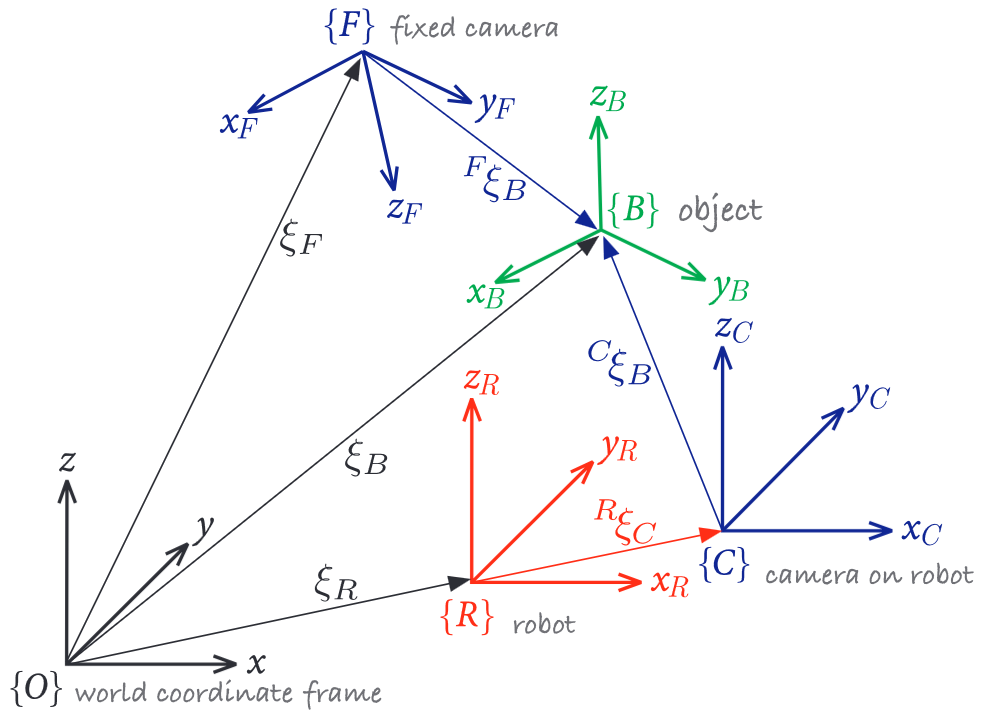
\includegraphics[width=0.9\textwidth]{multiple_frame_pose}}
  \caption{多个三维坐标系与相对位姿的例子}
  \label{fig:multiple_frame_pose}
\end{figure}
这些空间关系还可以用有向图来表示,如图\ref{fig:pose_directed_graph}。
\begin{figure}[htbp]
  \centerline{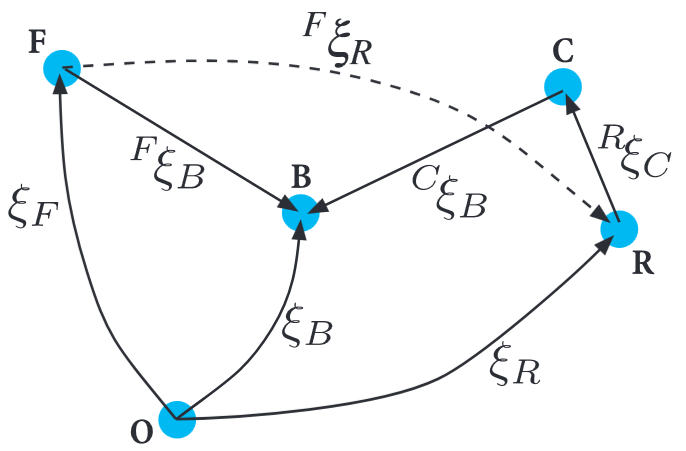
\includegraphics[width=0.9\textwidth]{pose_directed_graph}}
  \caption{有向图表示的空间关系}
  \label{fig:pose_directed_graph}
\end{figure}
  
\item{\textbf{特殊欧式群}}
  特殊欧式群(special Euclidean group),在二维和三维中分别记为SE(2)和SE(3)。
  群元素是位姿(即满足某种条件的2维或3维矩阵),它满足结合律,有单位元,逆元。
  记该群为 $\langle G,\oplus,0,\ominus\rangle$,其抽象的运算规则如下:
  \begin{itemize}
  \item {相对位姿可以把一个点在某个坐标系下的向量表示转换到另一个坐标系下},${}^Xp={}^X\xi_Y\cdot{}^Yp$。
  \item{位姿可以复合},${}^X\xi_Y\oplus{}^Y\xi_Z={}^X\xi_Z$。
  \item{零相对位姿,$0$}。
  \item{每个元素都有逆元},$\ominus{}^X\xi_Y={}^Y\xi_X$。
  \item{一些代数规则},
    $
    \xi\oplus0=\xi,\quad0\oplus\xi=\xi,\quad\xi\oplus(\ominus\xi)=0,\quad(\ominus\xi)\oplus\xi=0.
    $
  \item {复合运算不交换},$\xi_1\oplus\xi_2\ne\xi_2\oplus\xi_1$。
    一个例外是当$\xi_1\oplus\xi_2=0$时。
  \end{itemize}
  另外,该群具有执行代数的能力。
  一方面,群都满足消去律,所以可以化简等式。
  另一方面,可快速找到任意节点$X$相对于节点$Y$的位姿,步骤为:
  \begin{enumerate}
  \item 找到一条从$Y$到$X$的路径,在边上从左到右的写下相对位姿;
  \item 如果所经过的边与箭头方向相同则在前面冠以$\oplus$,否则冠以$\ominus$。
  \end{enumerate}
  例如,若要计算$R$相对于$F$的位姿${}^F\xi_R$,有多个路径可选。
  当选择$F,O,R$时,获得的相对位姿是$\ominus\xi_F\oplus\xi_R$。
  当选择$F,B,C,R$时,获得的相对位姿是$\oplus{}^F\xi_B\ominus{}^C\xi_B\ominus{}^R\xi_C$。
\item{\textbf{位姿$\xi$到底是什么?}}
  它是一种能够满足上述代数运算的任何数学对象。
  接下来会介绍。
  熟悉的概念包括向量等。
  其他的将是更奇特的数学对象,例如齐次变换、正交旋转矩阵、扭曲和四元数。
\end{itemize}

% ##################################################################################################
\section{二维情形}\label{sec:2D}

% \begin{table}[htbp]
%   \caption{Verilog files of the RISC-V Kernel} \label{tab:files}
%   \centering
%   \addtolength{\tabcolsep}{-0mm} % 控制列间距
%   \begin{tabular}{rrl}
%     \toprule[0.75pt]
%     File name & Lines & Description \\
%     \midrule[0.5pt]	
%     defines.v 		& 140 & global configurations and parameters\\
%     S011HD1P\_X32Y2D128\_BW.v & 32 & RAM behavior module \\
%     regfile.v 		& 208 & register file \\
%     SimTop4Soc.v 	& 192 & Simulation for SoC top module \\
%     \midrule[0.5pt]
%               & 5124 & \\ 
%     \bottomrule[0.75pt]
%   \end{tabular}
% \end{table}


% % ##################################################################################################
% \section{Experiment}\label{sec:experiment}
% a)	某实验A

% b)	某实验B


% % ##################################################################################################
% \section{Conclusion}\label{sec:conclusion}
% a)	Cache设计带来了好处

% b)	Cache的可扩展性设计

% c)	其他研究内容的引出


% % \section*{以下为一些工具}
% % \begin{align}
%   %   & ABCDEFGHIJKLMNOPQRSTUVWXYZ \label{eq:alphabet} \\
% %		& abcdefghijklmnopqrstuvwxyz \\
% %	& \alpha \beta \gamma \delta \epsilon \varepsilon \zeta \eta \theta \lambda \mu \nu \xi \pi \rho \sigma \tau \upsilon \phi \varphi \chi \psi \omega
% %	\end{align}
% %	
% %    \begin{align}
% %	 \begin{bmatrix}
% %		1 & 2 \\
% %		3 & 4 \\
% %	\end{bmatrix}
% %	 \begin{pmatrix}
% %	1 & 2 \\
% %	3 & 4 \\
% %	\end{pmatrix}
% %	 \begin{matrix}
% %	1 & 2 \\
% %	3 & 4 \\
% %	\end{matrix}
% %	\end{align}
% %
% %    \begin{equation}
% %	A_{t+1} = \arg\min_A \ \mathcal{L}(A,E_t,\Delta\tau_t,W_t,b_t), \nonumber
% %	\end{equation}
% %
% %    \begin{equation}
% %	\begin{aligned} \label{eq:rasl}
% %	\min_{A,E,\Delta \tau} \quad & \sum_{i=1}^{N}||A_i||_* + \lambda ||E_i||_1  \\
% %	\mathrm{s.t.} \quad & D_i \circ \tau_i + \sum_{k=1}^{n_i} J_{ik} \Delta \tau_i \epsilon_k \epsilon_k^T = A_i + E_i, \\
% %	& i = 1,2,\cdots,N.
% %	\end{aligned}
% %	\end{equation}
% %
% %    \begin{table}[htbp]
% %		\caption{Title of table} \label{tab:table}
% %		\centering
% %		\addtolength{\tabcolsep}{-0mm} % 控制列间距
% %		\begin{tabular}{ccccc}
% %			\toprule[0.75pt]	% package booktabs
% %			\multicolumn{4}{c}{table head} \\
% %			\midrule[0.5pt]	% package booktabs
% %			\multirow{4}{*}{text} & 1 & 2 & 3 & 4 \\  % package multirow
% %			& 5 & 6 & 7 & 8 \\
% %			\cmidrule[0.5pt]{2-4}	% package booktabs
% %			& 9 & 10 & 11 & 12 \\
% %			& 13 & 14 & 15 & 16 \\
% %			\bottomrule[0.75pt]	% package booktabs
% %		\end{tabular}
% %	\end{table}
% %    引用: Eq. \eqref{eq:alphabet}, Fig. \ref{figure:zju1},  \\
% %
% %
% %    \begin{algorithm}
% %		\caption{Title of the Algorithm}
% %		\label{algo:ref}
% %		\begin{algorithmic}[1]
% %			\REQUIRE some words.  % this command shows "Input"
% %			\ENSURE ~\\           % this command shows "Initialized"
% %			some text goes here ... \\
% %			\WHILE {\emph{not converged}}
% %			\STATE ... \\  % line number at left side
% %			\ENDWHILE
% %			\RETURN this is the lat part.  % this command shows "Output"
% %		\end{algorithmic}
% %	\end{algorithm}


% \bibliographystyle{plain}
% \bibliography{sample}
\end{document} 